%! Author = adnansiddiquei
%! Date = 19/03/2024

\section{Custom Degradation - Fashion MNIST Degradation}\label{sec:q2}
A fashion MNIST degradation was implemented to train the diffusion model to generate MNIST digits.
This section discusses the design of this model, the training process and a comparison of this model with the 3 models
trained in Section~\eqref{sec:q1bc}.

\subsection{Model Design}\label{subsec:model-design}
\begin{figure}[t]
    \centering
    
\includegraphics[width=0.8\textwidth]{figures/q2_encoding}
    \caption{The encoding process for the fashion MNIST diffusion model.}
    \label{fig:q2_encoding}
\end{figure}

The exact same CNN architecture was used as in Section~\eqref{sec:q1bc} to learn the diffusion process.
The primary differences were the \inlinecode{forward} and \inlinecode{sample} functions, with the sampling process
derived from Bansal et al., (2022)~\cite{bansal}.

The forward function worked in a similar way to the \inlinecode{DDPM} models.
Degradation was applied onto the training data using Equation~\eqref{eq:schedule}, where $\epsilon$ was a randomly
sampled fashion MNIST image instead of standard normal noise.
In this way, a similar system for noise schedules could be applied, and as such, the fashion MNIST degradation was
applied using the default noise schedule of $\beta_{t} = [10^{-4}, 0.02]$ in 1000 steps.
Everything else with regard to the training process remained identical to the DDPM models detailed in Section~\eqref{sec:q1bc}.

Unconditional sampling was used for the sampling process where a random fashion MNIST digit from the test set was chosen
as the initial image and MNIST digits were generated by iterating backwards through the diffusion process.
This reverse process was implemented using Algorithm 2 from Bansal et al., (2022)~\cite{bansal}.

\subsection{Model Training and Analysis}\label{subsec:model-training}
\begin{figure}[t]
    \centering
    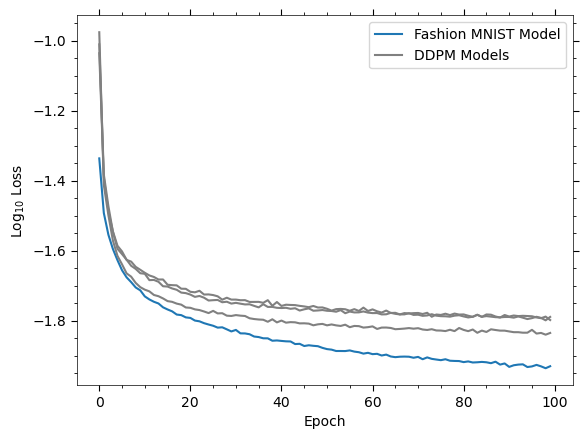
\includegraphics[width=0.8\textwidth]{figures/q2_training_loss}
    \caption{The training loss for the fashion MNIST diffusion model.
        The loss for the DDPM models from Section~\eqref{sec:q1bc} is also shown in grey for comparison.}
    \label{fig:q2_training_loss}
\end{figure}

\begin{figure}[t]
    \centering
    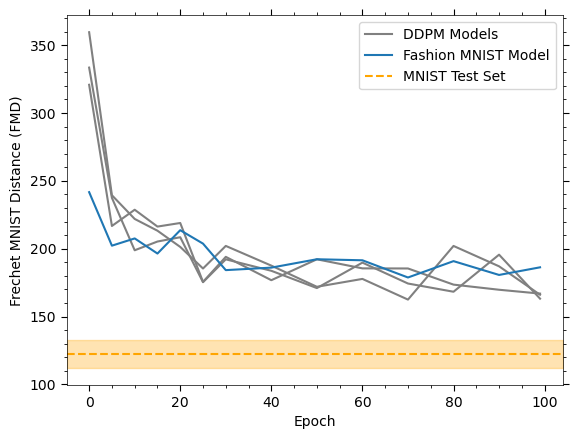
\includegraphics[width=0.8\textwidth]{figures/q2_fmd}
    \caption{The FMD values for the fashion MNIST diffusion model.
        The FMD values for the DDPM models from Section~\eqref{sec:q1bc} are also shown in grey for comparison.}
    \label{fig:q2_fmd}
\end{figure}

\begin{figure}[t]
    \centering
    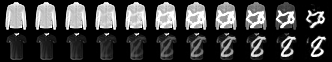
\includegraphics[width=0.8\textwidth]{figures/q2_decoding}
    \caption{The decoding process for the fashion MNIST diffusion model shown with two samples with the trained model.}
    \label{fig:q2_decoding}
\end{figure}

\begin{figure}[t]
    \centering
    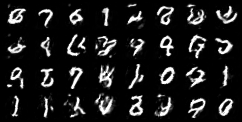
\includegraphics[width=0.8\textwidth]{figures/q2_samples_final}
    \caption{32 samples generated from the trained fashion MNIST diffusion model.}
    \label{fig:q2_samples_final}
\end{figure}

Figure~\eqref{fig:q2_samples_final} shows the training loss for the fashion MNIST diffusion model (FMDM) over 100 epochs, and
Figure~\eqref{fig:q2_fmd} shows the FMD for samples generated from the trained model at varyin epochs.
Whilst the train loss for the FMDM reached lower values than the DDPM models, the FMD values for all models were
not significantly different and inspecting the samples generated by the FMDM in Figure~\eqref{fig:q2_samples_final}
indicates no significant difference in the quality of the samples generated by the FMDM compared to the DDPM models.
It is also worth noting, whilst the FMDM had lower training loss, the loss criterion for both models were slightly
different in that the FMDM was trained to predict the input \inlinecode{x} given a degraded image, whilst the DDPM models
were trained to predict the noise added in the previous step.
Therefore, the loss curves are not as directly comparable as the FMD values are, which combined with the visual inspection,
indicate no significant difference between the two degradations.

Given that all models were allowed to train for sufficient time that the loss curve had plateaued, it is fair to conclude
that neither of these 4 models produce samples that are consistently realistic and visually similar to real MNIST
digits.
It is possible that more realistic sample could be generated with different (non-linear) noise schedules, or it is also
entirely possible that the current capacity of the CNN architecture is not sufficient to learn the diffusion process
for MNIST digits.
Further investigation would be required to assess which of these is the case, but it is likely that the latter is the
case.
